\section{Results}

% ==========================================
% 3. SECTION 3.1
% ==========================================
\subsection{Comparative Performance of Classical ML Across Feature Spaces}

We established a rigorous baseline for TgDHFR inhibitor prediction by evaluating classical machine learning ensembles across four molecular representations using a \TotalOuterFolds-fold nested cross-validation framework. The purely structural representation utilizing Morgan fingerprints (ECFP4, \MorganNFeaturesTotal\ bits) yielded the highest predictive performance ($R^2 = \MorganRTwoMean \pm \MorganRTwoStd$, MAE = \MorganMaeMean). To definitively rule out chance correlation, we subjected this optimized baseline to a 100-iteration y-randomization protocol. The permuted models collapsed to a mean $R^2$ of $\YRandomMeanRTwo \pm \YRandomStdRTwo$, generating a massive statistical separation from the true predictive baseline ($Z = \YRandomZScore$). This confirms the ensemble maps genuine physicochemical relationships rather than memorizing noise.

Figure~\ref{fig:nested_cv_boxplot} illustrates the distribution of explained variance across all evaluated feature spaces. Within the Morgan fingerprint space, architectural selection exhibited severe fluidity. Rather than converging on a single dominant hierarchy, five distinct architectures tied as the most frequently selected configurations (\MorganStability\% each, 3/25 folds): LGBM+XGB+SVM, RF+SVM, RF+XGB+SVM, SVM, and XGB+SVM+kNN. This distribution confirms that while aggregated predictive performance remains robust across the outer folds, the inherent data sparsity of the \NCompounds-compound benchmark prevents the inner optimization loop from isolating a universally superior stacking hierarchy.

\begin{figure}[htbp]
	\centering
	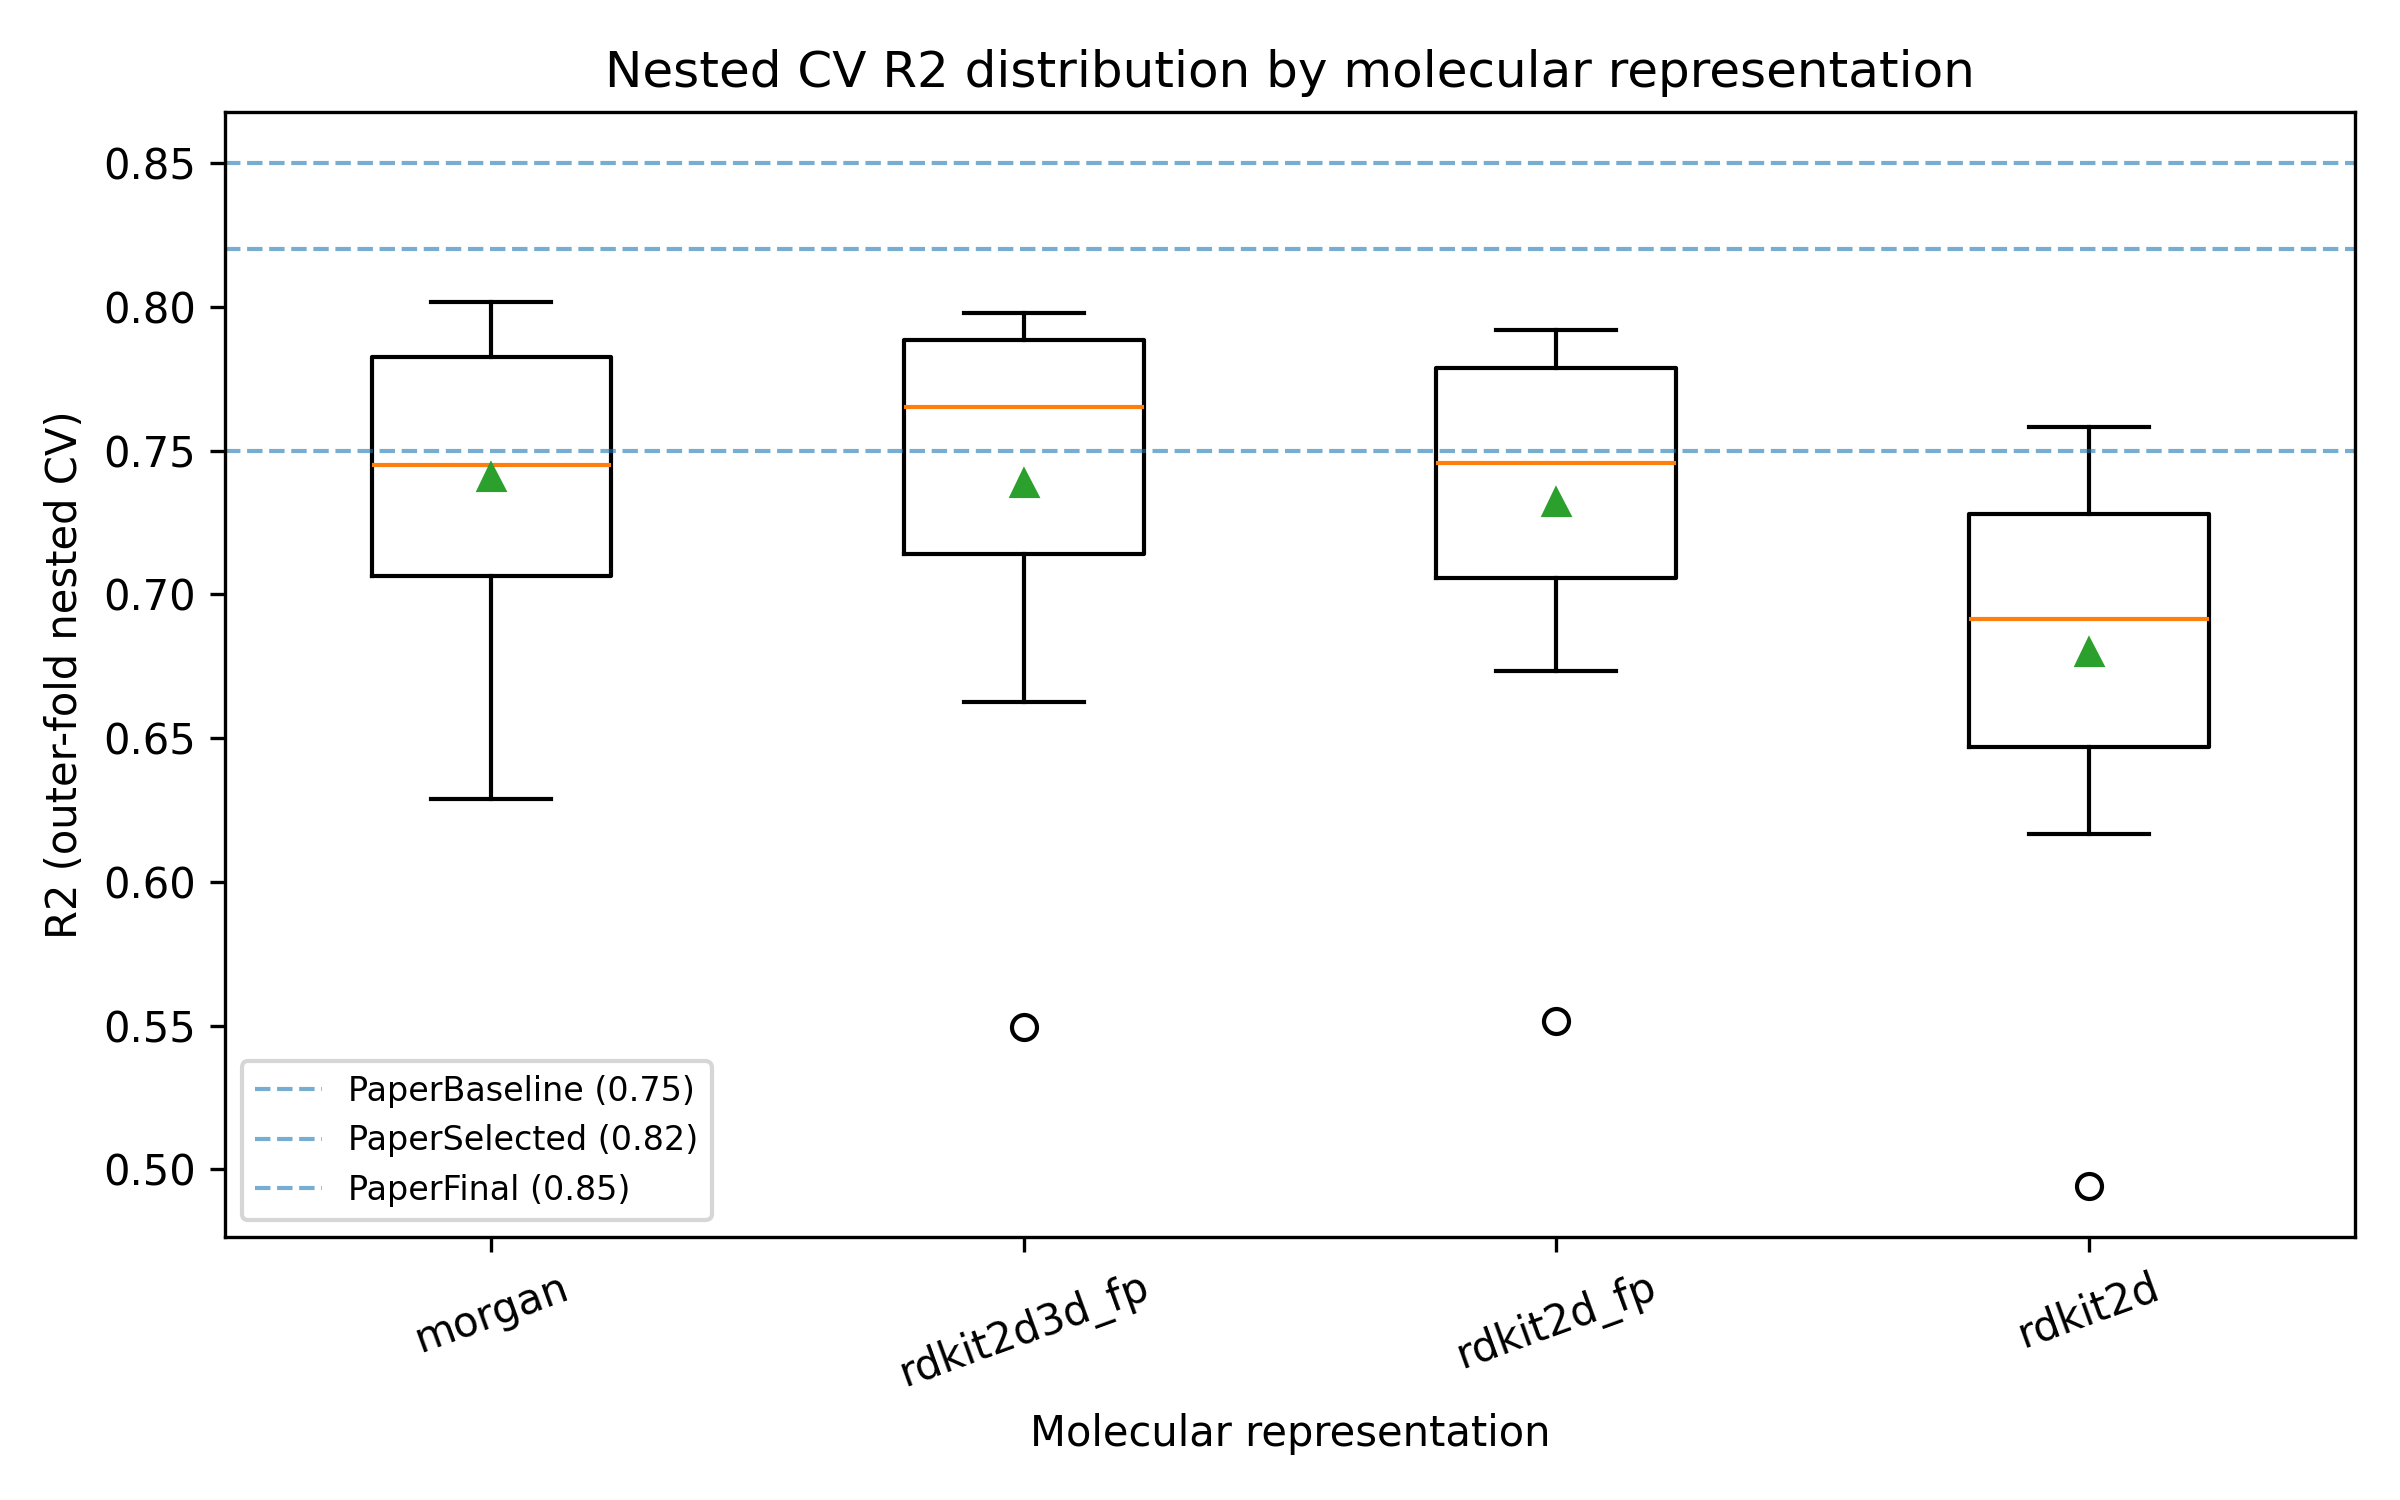
\includegraphics[width=0.8\textwidth]{figures/r2_by_representation_boxplot.png}
	\caption{Nested cross-validation $R^2$ distributions across four molecular representations. The purely structural Morgan fingerprint representation demonstrates equivalent predictive capacity to highly engineered 3D descriptors, establishing a robust classical baseline.}
	\label{fig:nested_cv_boxplot}
\end{figure}

Escalating feature complexity failed to yield commensurate predictive gains. Integrating RDKit 2D descriptors with Morgan fingerprints (analogous to the original study's ``2D/FP'' model) produced an $R^2$ of $\RdkitTwoDFpRTwoMean \pm \RdkitTwoDFpRTwoStd$ and an MAE of \RdkitTwoDFpMaeMean. The most complex representation, incorporating 3D geometric descriptors derived from ETKDGv3 embedding and MMFF94s optimization (analogous to the ``2D/3D/FP'' model), attained an $R^2$ of $\RdkitTwoDThreeDFpRTwoMean \pm \RdkitTwoDThreeDFpRTwoStd$ and an MAE of \RdkitTwoDThreeDFpMaeMean. A paired t-test comparing the purely structural Morgan fingerprint ensemble against the highly engineered 2D/3D/FP model revealed no statistically significant difference in explained variance ($t = \PairedTTestStat$, $p = \PairedTTestP$). To rigorously assess error magnitude differences while avoiding pseudoreplication artifacts, we applied a Nadeau-Bengio corrected paired t-test to the cross-validated MAE distributions. This confirmed the variance in absolute error lacks statistical significance ($t = \CorrectedTStat$, $p = \CorrectedTP$). These results indicate that conformational 3D featurization offers no measurable predictive advantage for this specific benchmark. Conversely, relying exclusively on 2D physicochemical descriptors severely degraded performance ($R^2 = \RdkitTwoDRTwoMean \pm \RdkitTwoDRTwoStd$, MAE = \RdkitTwoDMaeMean). Topological fingerprints act as the primary drivers of predictive capacity.

We benchmarked our highest-performing classical model against the incremental progression reported in the original study to contextualize the computational cost-benefit ratio of advanced statistical techniques (Table~\ref{tab:methodological_comparison}). Our classical stacking ensemble trained solely on Morgan features ($R^2 = \MorganRTwoMean$) performed comparably to their unselected 2D/3D/FP baseline model ($R^2 = \PaperBaselineRTwo$). Evaluated under a Nadeau-Bengio corrected one-sample $t$-test, this variance lacks statistical significance ($t = \TStatMorganVsPaperBaseline$, $p = \PValueMorganVsPaperBaseline$). Furthermore, our baseline 95\% bootstrap confidence interval $[\ExpARTwoCILow, \ExpARTwoCIHigh]$ strictly encompasses the literature baseline, confirming statistical parity. 

However, the literature model utilizing permutation importance-based feature selection ($R^2 = \PaperSelectedRTwo$) represents a statistically significant improvement over our unselected baseline ($t = \TStatMorganVsPaperSelected$, $p = \PValueMorganVsPaperSelected$), attributable to the supervised isolation of pharmacophoric signals. Similarly, the original study's final data-augmented deep neural network ensemble ($R^2 = \PaperFinalRTwo$) resides outside our baseline 95\% CI, representing a statistically significant deviation ($t = \TStatMorganVsPaperFinal$, $p = \PValueMorganVsPaperFinal$). These comparative results isolate the true source of predictive gains in this low-data regime. Achieving a competitive baseline performance ($R^2 \approx \PaperBaselineRTwo$) does not require computationally expensive 3D descriptors or complex neural network architectures; simple 2D fingerprints paired with classical machine learning algorithms suffice. The performance gaps between our baseline and the original study's advanced models directly quantify the impact of supervised feature selection and synthetic data augmentation rather than inherent architectural superiority.

\begin{table}[htbp]
	\centering
	\caption{Methodological comparison isolating the performance impact of architectural complexity, descriptor dimensionality, and data augmentation in TgDHFR bioactivity prediction.}
	\label{tab:methodological_comparison}
	\begin{tabular}{lllc}
		\toprule
		\textbf{Model Framework} & \textbf{Descriptors} & \textbf{Data Augmentation} & \textbf{Test $R^2$ (mean $\pm$ std)} \\
		\midrule
		Current Study (Classical Ensemble) & ECFP4 (2D) & None & \MorganRTwoMean $\pm$ \MorganRTwoStd \\
		Baseline \cite{karimova2025} & 2D/3D/FP & None & \PaperBaselineRTwo \textsuperscript{a} \\
		Augmented Final Model \cite{karimova2025} & 2D/3D/FP (Selected) & Gaussian Noise & \PaperFinalRTwo \textsuperscript{a} \\
		\bottomrule
		\multicolumn{4}{l}{\footnotesize \textsuperscript{a} Standard deviation not reported (NR) in the original study.}
	\end{tabular}
\end{table}
% ==========================================
% 3. SECTION 3.2
% ==========================================
\subsection{Benchmarking Tree-Based Ensembles Against Graph Neural Networks}

Graph Neural Networks (GNNs) dominate molecular property prediction by extracting representations directly from graph topologies. Their predictive utility, however, degrades sharply under data scarcity. To evaluate whether deep representation learning offers intrinsic advantages for the TgDHFR dataset (\NCompounds\ compounds), we benchmarked our optimal classical ensemble against a Directed Message Passing Neural Network (D-MPNN) using the Chemprop framework.

The D-MPNN yielded a cross-validated out-of-sample $R^2$ of $\ChemPropDMPNNFoldRTwoMean \pm \ChemPropDMPNNFoldRTwoStd$ and a Mean Absolute Error of \ChemPropDMPNNFoldMae. This network failed to match the classical stacking ensemble operating on pre-computed Morgan fingerprints ($R^2 = \MorganRTwoMean \pm \MorganRTwoStd$). This performance deficit stems directly from data scarcity and methodological asymmetry. The classical models underwent extensive hyperparameter optimization and architecture selection via the nested cross-validation pipeline. In contrast, the D-MPNN was evaluated using baseline hyperparameters without an equivalent exhaustive tuning phase. Restricted to \NCompounds\ training instances, the unoptimized D-MPNN cannot learn graph convolutions capable of surpassing the predictive baseline established by fixed, topological ECFP4 descriptors.

This convergence plateau provides contextual validation for the methodologies in the original study \cite{karimova2025}. The poor performance of the unaugmented D-MPNN explains the prior reliance on heavy statistical interventions—specifically, Gaussian data augmentation—to force predictive accuracy ($R^2 = \PaperFinalRTwo$, $p < 0.001$). Evaluated on unaugmented, data-limited chemical spaces, architectural complexity does not guarantee superior generalization. Classical tree-based ensembles utilizing fixed molecular descriptors remain the most robust, parsimonious, and computationally efficient alternative. Figure~\ref{fig:gnn_comparison} details the comparative performance across all baseline models and the GNN.

\begin{figure}[htbp] 
	\centering
	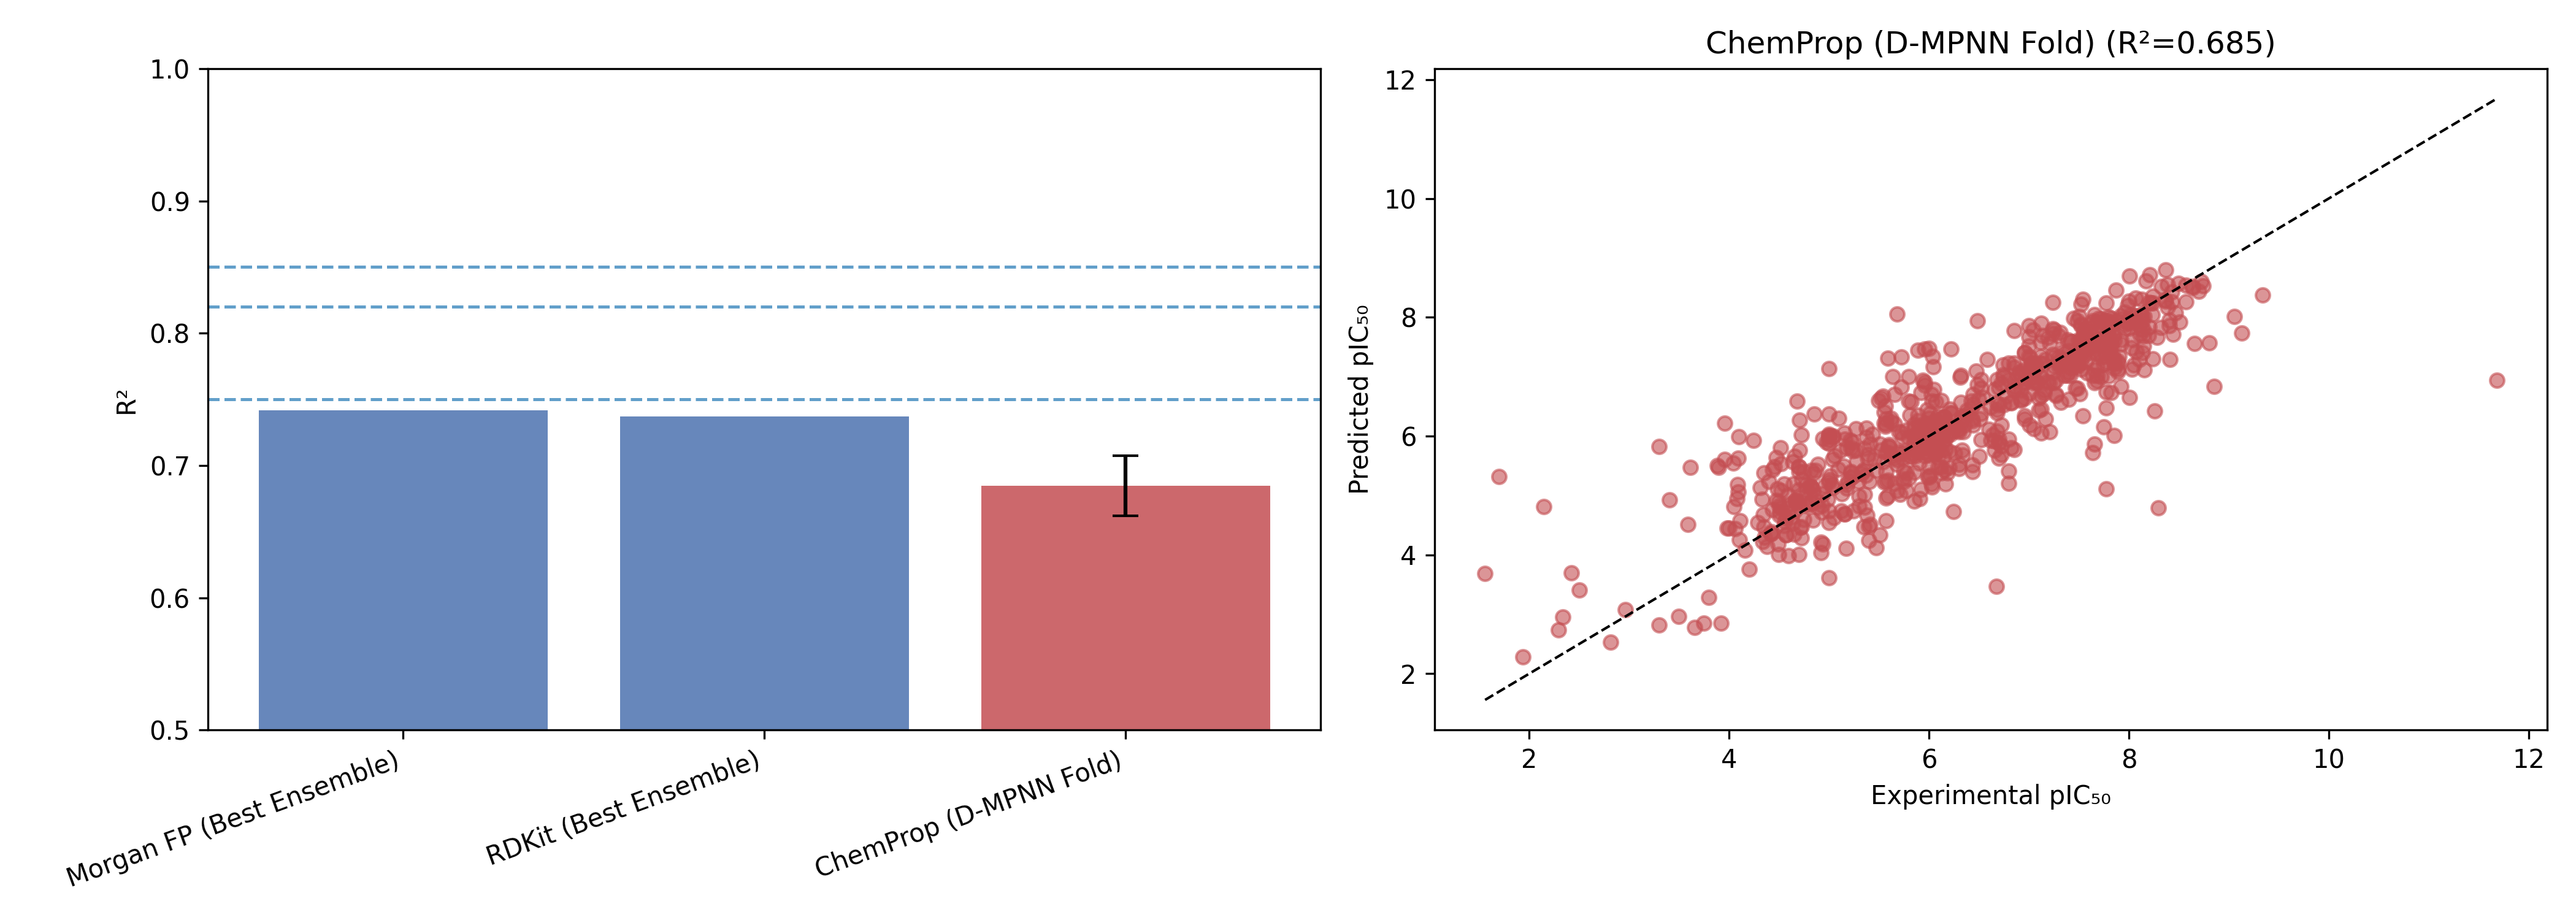
\includegraphics[scale=0.45]{figures/gnn_comparison.png} 
	\caption{Comparative predictive performance of classical machine learning ensembles, the Chemprop D-MPNN, and the original study's baseline and final models. The scatter plot details the predicted versus experimental $pIC_{50}$ values for the D-MPNN.}
	\label{fig:gnn_comparison} 
\end{figure}

% ==========================================
% 3. SECTION 3.3
% ==========================================
\subsection{Virtual Screening and Prioritization of FDA-Approved Candidates}

Transitioning from theoretical benchmarking to applied therapeutic discovery required deploying the optimized classical ensemble (\WinnerMode, $R^2 = \WinnerRTwoMean$) against a curated library of FDA-approved compounds. Prior to evaluating uncharacterized chemical spaces, the pipeline's predictive reliability underwent quantification using established TgDHFR inhibitors retained within the dataset. The algorithm recovered these internal controls with high fidelity. It assigned a predicted pIC$_{50}$ of 6.3259 to pyrimethamine (experimental: 6.56, absolute error: 0.2341) and 5.6352 to trimethoprim (experimental: 5.57, absolute error: 0.0652). This empirical alignment confirms the ensemble's capacity to interpolate bioactivity accurately within its defined applicability domain. To visualize this chemical space alignment, Principal Component Analysis (PCA) of the Morgan fingerprints confirmed that the prioritized FDA candidates fall strictly within the dense regions of the training distribution (Figure S1).

Following unsupervised Isolation Forest filtering to exclude structural outliers, the virtual screening protocol prioritized candidates based on absolute predicted potency and multi-objective ligand efficiency. Table~\ref{tab:fda_candidates} delineates the top ten prioritized compounds. Classic antifolate analogs—specifically methotrexate, trimetrexate, and folic acid—dominated the upper echelon of absolute affinity, all exceeding a predicted pIC$_{50}$ of 7.0. Absolute potency, however, frequently scales with molecular weight. This size dependency can artificially inflate binding scores and obscure the intrinsic thermodynamic quality of the underlying scaffold.

Correcting for physicochemical load via heavy-atom and molecular weight penalties revealed a distinct hierarchy of efficient binders. Smaller architectures demonstrated vastly superior atomic utilization. Pyrimethamine (LE = 0.51, BEI = 25.43), the potassium-sparing diuretic triamterene (LE = 0.48, BEI = 26.07), and the phenothiazine derivative methylene blue (LE = 0.45, BEI = 21.60) emerged as the most structurally optimized candidates. Triamterene and methylene blue provide particularly compelling repurposing profiles. They achieve robust predicted bioactivities while maintaining exceptional ligand efficiency indices, indicating highly complementary interactions with the TgDHFR catalytic pocket relative to their minimal steric footprints.

\begin{table}[htbp]
	\centering
	\caption{Top 10 FDA-approved candidates predicted by the classical ML model, ranked by predicted pIC$_{50}$ and evaluated across standard ligand efficiency metrics.}
	\label{tab:fda_candidates}
	\begin{tabular}{llccccc}
		\toprule
		\textbf{Rank} & \textbf{Compound Name} & \textbf{Predicted pIC$_{50}$} & \textbf{LE} & \textbf{BEI} & \textbf{LLE} & \textbf{SEI} \\
		\midrule
		1 & Methotrexate & 7.5678 & 0.31 & 16.65 & 7.30 & 3.59 \\
		2 & Trimetrexate Glucuronate (CID 54949) & 7.3351 & 0.25 & 13.02 & 7.88 & 2.90 \\
		3 & Trimetrexate Glucuronate (CID 336805) & 7.3351 & 0.25 & 13.02 & 7.88 & 2.90 \\
		4 & Folic Acid & 7.0830 & 0.30 & 16.05 & 7.13 & 3.32 \\
		5 & Methylene Blue & 6.9091 & 0.45 & 21.60 & 7.41 & 36.10 \\
		6 & Bendamustine Hydrochloride & 6.8859 & 0.39 & 17.44 & 3.20 & 11.39 \\
		7 & Fentanyl Citrate & 6.8673 & 0.25 & 12.99 & 3.98 & 4.41 \\
		8 & Ivabradine & 6.8497 & 0.28 & 14.62 & 3.54 & 11.33 \\
		9 & Ivabradine Hydrochloride & 6.8492 & 0.27 & 13.56 & 3.12 & 11.33 \\
		10 & Trifarotene & 6.8311 & 0.28 & 14.86 & 0.84 & 9.76 \\
		\bottomrule
	\end{tabular}
\end{table}
% ==========================================
% 3. SECTION 3.4
% ==========================================
\subsection{Integrated ML-docking consensus filtering and false-positive mitigation}

Standalone virtual screening methodologies generate false-positive artifacts. To mitigate this vulnerability, we implemented an orthogonal consensus filtering pipeline integrating ligand-based machine learning predictions with physics-based molecular docking. Spearman's rank correlation coefficient evaluated the global agreement between ML-predicted $pIC_{50}$ values and AutoDock Vina binding energies across the prioritized subset ($N = \DockNTotal$). This non-parametric approach ($\rho = \DockSpearmanRho$, $p = \DockSpearmanP$) handles restricted sample sizes and isolates monotonic trends without assuming linear dependencies between topological bioactivity interpolation and thermodynamic scoring.

The negative correlation confirms that higher predicted potencies trend with stronger binding energies. The absence of statistical significance ($p > 0.05$) validates the methodological design: two-dimensional ligand-based machine learning and three-dimensional physics-based docking capture fundamentally orthogonal aspects of molecular interaction. The ML ensemble interpolates bioactivity from topological patterns within the training distribution, whereas Vina calculates thermodynamic stability via spatial complementarity and electrostatic interactions. Relying on either method in isolation exposes the screening process to distinct classes of false positives.

The consensus approach identified and eliminated these methodological artifacts. Bisacodyl perfectly illustrates a physics-based false positive. It exhibited strong thermodynamic binding energies during structural validation ($\Delta G = -8.82\text{ kcal/mol}$), driven by the spurious accommodation of its flexible, hydrophobic scaffold within the binding pocket. The classical ML model, however, correctly assigned a low predicted affinity ($pIC_{50} = 5.25$) to this compound, vetoing its progression. Conversely, the ML model generated exactly \DockNDiscordant\ false positives; every candidate exceeding the ML potency threshold also satisfied the stringent docking energy criteria. Dual validation thus prevents the misallocation of experimental resources toward single-method screening artifacts.

Orthogonal docking isolated exactly \DockNValidated\ consensus hits from the \DockNTotal\ evaluated compounds that satisfied both the ML potency threshold ($pIC_{50} > 6.5$) and the stringent docking energy criteria ($\Delta G < -8.0\text{ kcal/mol}$). These validated hits are folic acid ($\Delta G = -8.62\text{ kcal/mol}$), methotrexate ($\Delta G = -8.68\text{ kcal/mol}$), pralatrexate ($\Delta G = -9.43\text{ kcal/mol}$), and triamterene ($\Delta G = -8.05\text{ kcal/mol}$). The primary consensus candidate, \DockBestCandidate, demonstrated a strong ML-predicted $pIC_{50}$ of \DockBestMLpIC\ alongside the most favorable docking score of \DockBestDockScore\ kcal/mol.

This lightweight, classical pipeline matches the statistical performance of unaugmented deep learning models while discovering biologically viable, physics-validated inhibitors. Isolating high-confidence repurposing candidates without synthetic data generation or 3D feature engineering yields a superior computational cost-benefit ratio for practical drug discovery in low-data regimes.